\documentclass{article}
\usepackage{amsmath}
\usepackage{amssymb}
\usepackage{graphicx}
\usepackage{hyperref}
\usepackage[version=4]{mhchem}


\begin{document}
\section*{Problem}
The lengths of the three sides of a triangle are consecutive positive integers. The largest angle of the triangle is two times of the smallest angle. What is the largest side of the triangle?\\
\centering
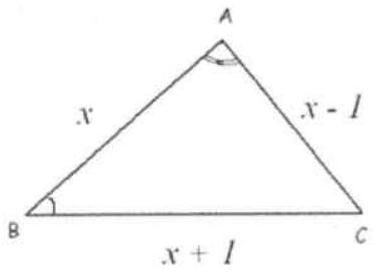
\includegraphics[width=\textwidth]{images/066(3).jpg}

\section*{Solution}
6.
Method 1: Let \(\angle A\) be the largest angle and \(\angle B\) be the smallest angle.\\
Draw the angle bisector of \(\angle A\) to meet \(B C\) at \(D . \angle \mathrm{A}\) is twice \(\angle B\). We know that \(\angle 2=\angle 3, \angle A D C=\angle 1+\angle 3=\angle A\). \(\triangle C A D \sim \triangle C B A\).\\
\centering
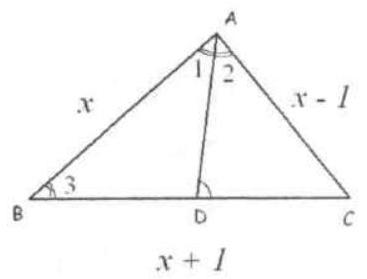
\includegraphics[width=\textwidth]{images/072(1).jpg}

We have: \(\frac{C D}{A C}=\frac{A C}{B C} \quad \Rightarrow \quad C D=\frac{A C^{2}}{B C}\)

According to the angle bisector theorem, we get:\\
\(\frac{A B}{B D}=\frac{A C}{C D} \quad \Rightarrow \quad \frac{C D}{B C-C D}=\frac{A C}{A B}\)\\
Separate \(C D\) to get: \(C D=\frac{A C \times B C}{A B+A C}\)\\
Substitute (2) into (1), \(\frac{A C^{2}}{B C}=\frac{A C \times B C}{A B+A C} \quad \Rightarrow \quad \frac{A C}{B C}=\frac{B C}{A B+A C}\)\\
\(\Rightarrow \quad \frac{x-1}{x+1}=\frac{x+1}{2 x-1} \quad \Rightarrow \quad x^{2}-5 x=0 \quad \Rightarrow \quad x=5\)\\
The largest side is \(x+1=6\).

Method 2: Extend \(C A\) to \(D\) such that \(A D=A B\). Then \(\angle 1=\angle 2\) and \(\angle C A B=\) \(2 \angle 2\). We are given that \(\angle C A B=2 \angle A B C\), so \(\angle 2=\angle A B C\) and \(\triangle A B C \sim \triangle B D C\).\\
\(\frac{x-1}{x+1}=\frac{x+1}{x-1+x} \quad \Rightarrow \quad(x-1)(2 x-1)=(x+1)^{2}\)\\
\(\Rightarrow \quad x^{2}-5 x=0 \quad \Rightarrow \quad x=5 \quad \Rightarrow \quad x+1=6\).

Method 3: We have the following theorem: In \(\triangle A B C\), if \(\angle A=\)\\
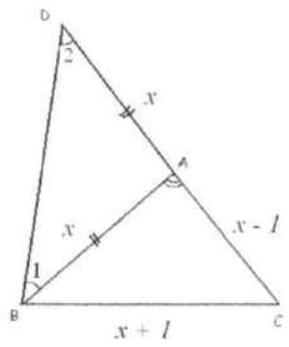
\includegraphics[width=\textwidth]{images/073.jpg} \(2 \angle B\), then \(a^{2}=b^{2}+b c\)\\
\(a=(x+1), b=(x-1)\), and \(c=x\)

\[
\begin{aligned}
& (x+1)^{2}=(x-1)^{2}+(x-1) x \Rightarrow x^{2}-5 x=0 \Rightarrow x=5 \\
& \Rightarrow \quad x+1=6 .
\end{aligned}
\]

Draw the height of the figure (especially when area calculation is involved).
\[
\longmapsto
\]

\begin{center}
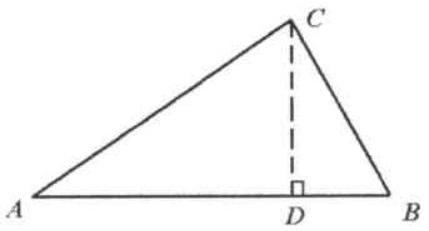
\includegraphics[width=\textwidth]{images/074.jpg}
\end{center}

Draw the height to hypotenuse of a right triangle
In triangle \(A B C, \angle A C D=90^{\circ}\), Draw \(C D \perp A B\). \(D\) is the feet of the perpendiculars to \(A B\) from \(C\).\\
Then \(\triangle A B C \sim \triangle A C D \sim \triangle C B D\).\\
\centering
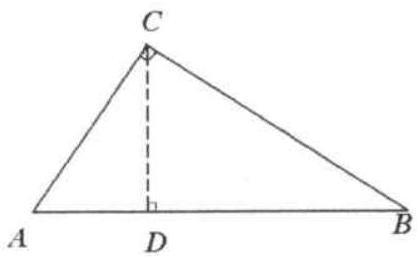
\includegraphics[width=\textwidth]{images/074(1).jpg}

Draw the second height of the figure when one height is shown.
In triangle \(A B C, A D \perp B C\). \(D\) is the feet of the perpendiculars to \(B C\) from \(A\). Draw \(B E \perp A C\). \(E\) is the feet of the perpendiculars to \(A C\) from B. \(A D\) meets \(B C\) at \(F\).

\[
\angle C B E=\angle C A D, \angle A F E=\angle C=\angle B F D .
\]

\begin{center}
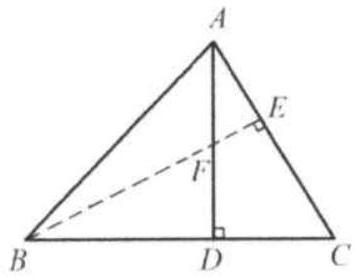
\includegraphics[width=\textwidth]{images/074(3).jpg}
\end{center}

Draw two heights of trapezoid from the short base to the long base.
In trapezoid \(A B C D, A B / / D C\). Draw \(A E\) and \(B F\) such that \(A E \perp D C, B F \perp D C\). As shown in the figure to the right,\\
\(A E=B F, A B=E F\).\\
\(D F+C E=D C+E F=D C+A B\).\\
\centering
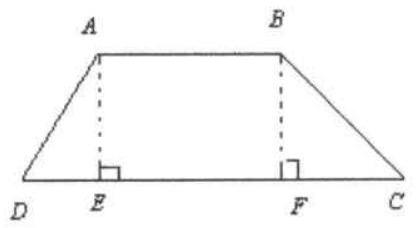
\includegraphics[width=\textwidth]{images/074(2).jpg}

\section*{Chapter 4 Draw the Auxiliary lines with Perpendicular Lines}

\end{document}
